\section{File upload}
\paragraph{Vulnerabilidad} El objetivo de este ataque es aprovecharse de una incorrecta
configuración de los permisos de la web, de tal forma que logremos ejecutar una función 
en php subiendo a la web un fichero y ejecutándolo.
\paragraph{Nivel bajo} En esta página nos permite únicamente subir un archivo, por lo que será nuestro único
punto de ataque. Para realizar el ataque escogimos un archivo que ejecute un {\it reverse shell} \cite{reverseshell}, ya que podríamos
poner simplemente una función que muestre un hola por pantalla, pero no sería tan divertido. 
Una vez subido el archivo la propia web nos indica donde se encuentra, tal y como muestra la figura \ref{fig:upload}.
\begin{figure}[ht!]
    \centering
    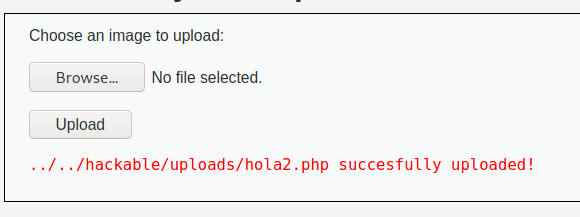
\includegraphics[width=14cm]{img/upload/succes.png}
    \caption{Reverse shell subido correctamente}
    \label{fig:upload}
\end{figure}
El siguiente paso sería ejecutarlo desde el navegador, para ello solo habría que poner 
la ruta obtenida en la barra de navegación. Tras esto dará la sensación que la página está colgada, pero únicamente esta a la espera 
de que establezcamos conexión desde un terminal, para ello ejecutamos
\begin{lstlisting}
    nc -lvp 7777
\end{lstlisting} 
y tendremos acceso a un {\it shell} en la página web como muestra la figura \ref{fig:reverseshell}
\begin{figure}[ht!]
    \centering
    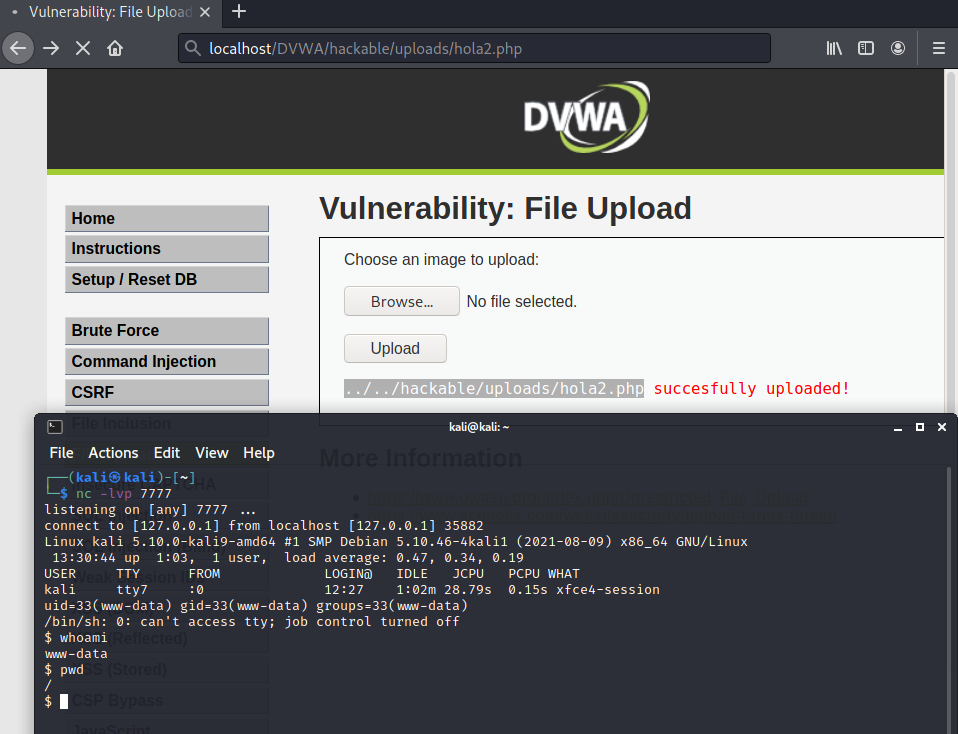
\includegraphics[width=14cm]{img/upload/low.png}
    \caption{ejecución de un reverse shell dentro de la web}
    \label{fig:reverseshell}
\end{figure} 
Posiblemente no nos funcione este ataque en niveles superiores dado que no nos permitirán subir scripts o 
no nos darán permisos de ejecución.
\paragraph{Nivel medio} Para este nivel probamos el mismo procedimiento para ver donde
habían implementado las contra medidas. Al tratar de subir el archivo nos dio error, indicando que
únicamente se pueden subir imágenes como se ve en la figura \ref{fig:onlyimages}.
\begin{figure}[ht!]
    \centering
    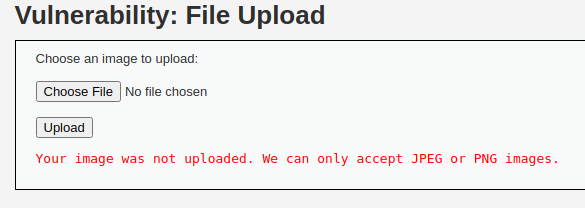
\includegraphics[width=14cm]{img/upload/only images.png}
    \caption{error al subir el reverse shell}
    \label{fig:onlyimages}
\end{figure} 
Tras buscar como se implementa esta contra medida vimos que en la cabecera de la petición,
se indica el tipo archivo que es, por lo que si subimos el archivo indicando en la petición que es 
una imagen posiblemente nos permitirá subirlo. Para ello consideramos utilizar {\it Burp suite}, una herramienta
preinstalada en Kali que es capaz de capturar las peticiones en un proxy, de tal forma que podemos tanto
observarlas como modificarlas.
\paragraph{} Lo primero que hicimos fue lanzar el {\it proxy} en {\it Burp suite}, clicando en la opción de 
{\it proxy} y después en abrir navegador tal y como se muestra en la figura \ref{fig:burp}.
\begin{figure}[ht!]
    \centering
    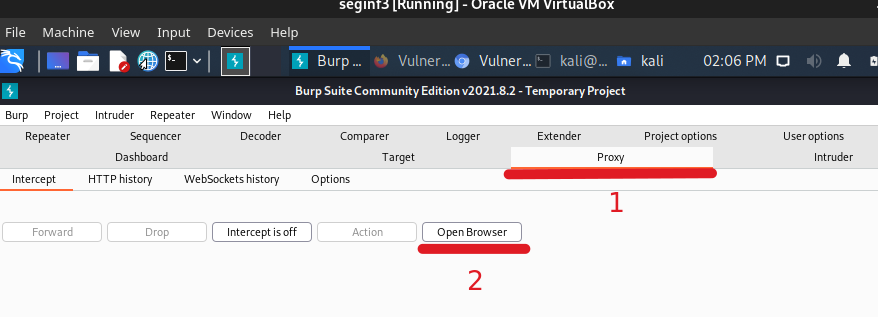
\includegraphics[width=14cm]{img/upload/burp.png}
    \caption{Abrir proxy en burp suite}
    \label{fig:burp}
\end{figure} 
Esto nos abrió una ventana de Chromiun desde la cual accedimos a la aplicación web. Una vez ahí volvimos a subir el archivo, pero en vez
de dar error se bloqueó a la espera de que el {\it proxy} permita continuar a la petición. En la figura \ref{fig:appphp} se muestra la petición
capturada, la cual indica que el tipo de archivo es un script php. Desde {\it Burp suite} modificamos la petción de tal forma que quede como
la figura \ref{fig:mod} y le damos a continuar petición. El resultado es satisfactorio obteniendo el mismo resultado que en la figura \ref{fig:upload}. Se acabo el 
procedimiento conectando con el reverse shell.
\begin{figure}[ht!]
    \centering
    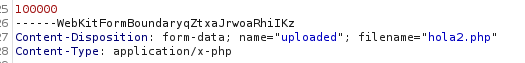
\includegraphics[width=14cm]{img/upload/appphp.png}
    \caption{Petición capturada}
    \label{fig:appphp}
\end{figure} 
\begin{figure}[ht!]
    \centering
    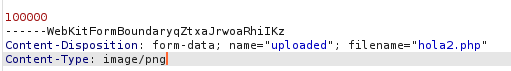
\includegraphics[width=14cm]{img/upload/content image.png}
    \caption{Petición modificada}
    \label{fig:mod}
\end{figure} 

Este ataque fallará en niveles más altos dado que posiblemente no limite la comprobación a la 
cabecera de la petición.

